\documentclass{standalone}
\usepackage{tikz}
\usetikzlibrary{patterns, positioning}


\begin{document}
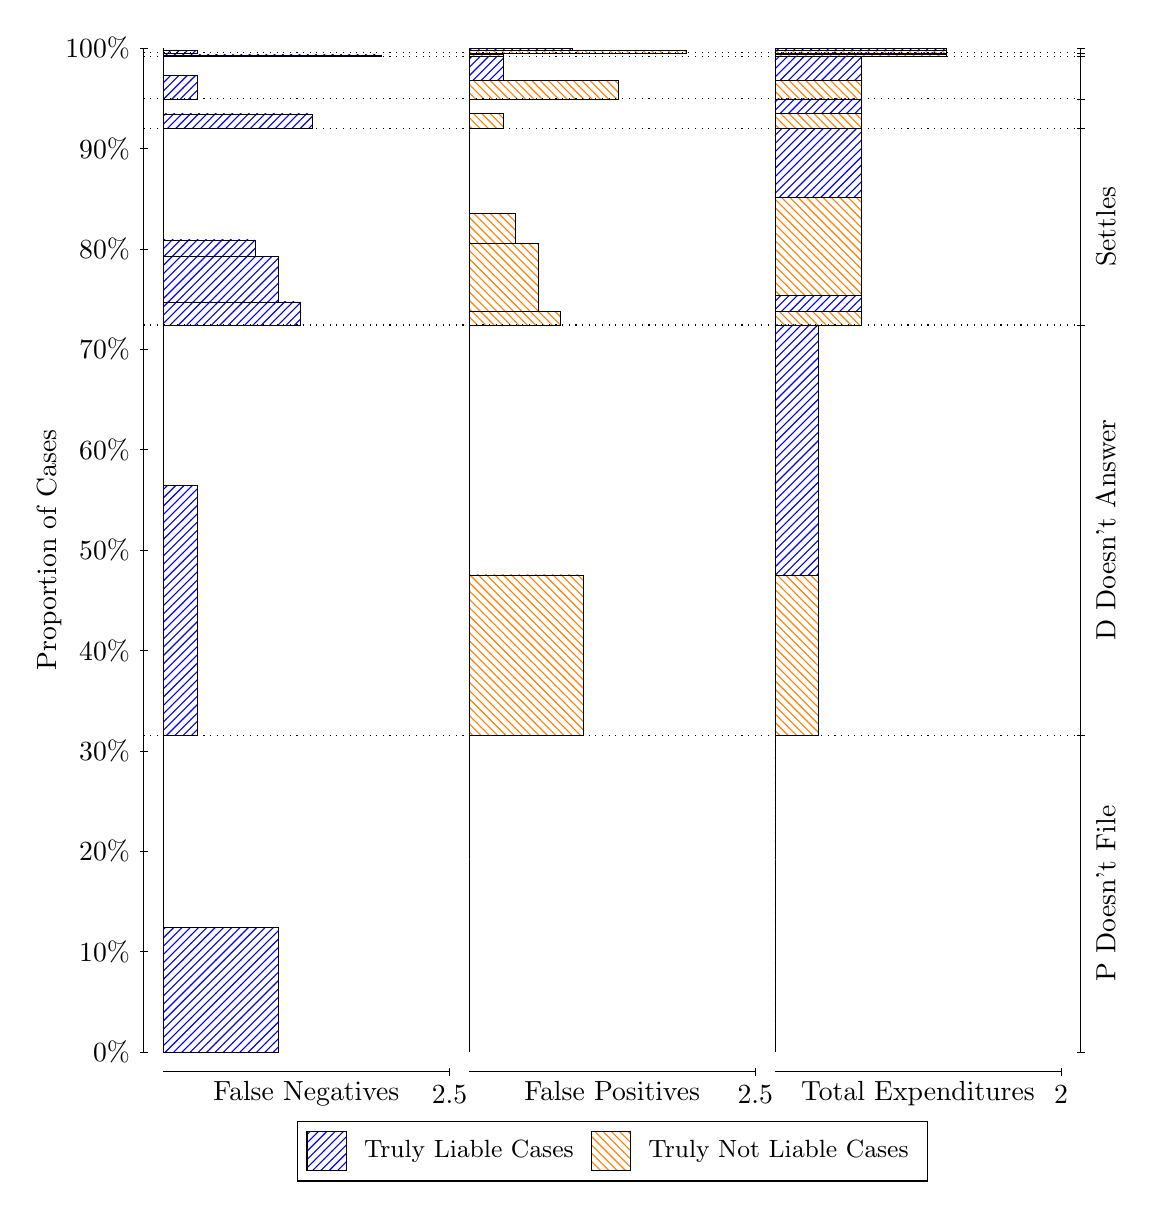
\begin{tikzpicture}
\draw[black, very thin] (1.5,1.75) -- (1.5,14.5);
\node[rotate=90, text=black, anchor=center] at (0.3, 8.125) {Proportion of Cases};
\draw[black, very thin] (1.45,1.75) -- (1.55,1.75);
\node[text=black, anchor=east] at (1.45, 1.75) {0\%};
\draw[black, very thin] (1.45,3.025) -- (1.55,3.025);
\node[text=black, anchor=east] at (1.45, 3.025) {10\%};
\draw[black, very thin] (1.45,4.3) -- (1.55,4.3);
\node[text=black, anchor=east] at (1.45, 4.3) {20\%};
\draw[black, very thin] (1.45,5.575) -- (1.55,5.575);
\node[text=black, anchor=east] at (1.45, 5.575) {30\%};
\draw[black, very thin] (1.45,6.85) -- (1.55,6.85);
\node[text=black, anchor=east] at (1.45, 6.85) {40\%};
\draw[black, very thin] (1.45,8.125) -- (1.55,8.125);
\node[text=black, anchor=east] at (1.45, 8.125) {50\%};
\draw[black, very thin] (1.45,9.4) -- (1.55,9.4);
\node[text=black, anchor=east] at (1.45, 9.4) {60\%};
\draw[black, very thin] (1.45,10.675) -- (1.55,10.675);
\node[text=black, anchor=east] at (1.45, 10.675) {70\%};
\draw[black, very thin] (1.45,11.95) -- (1.55,11.95);
\node[text=black, anchor=east] at (1.45, 11.95) {80\%};
\draw[black, very thin] (1.45,13.225) -- (1.55,13.225);
\node[text=black, anchor=east] at (1.45, 13.225) {90\%};
\draw[black, very thin] (1.45,14.5) -- (1.55,14.5);
\node[text=black, anchor=east] at (1.45, 14.5) {100\%};

\draw[black, very thin] (13.4,1.75) -- (13.4,14.5);
\draw[black, very thin] (13.35,1.75) -- (13.45,1.75);
\node[anchor=west] at (13.35, 1.75) {};
\draw[black, very thin] (13.35,5.773) -- (13.45,5.773);
\node[anchor=west] at (13.35, 5.773) {};
\draw[black, very thin] (13.35,10.983) -- (13.45,10.983);
\node[anchor=west] at (13.35, 10.983) {};
\draw[black, very thin] (13.35,13.476) -- (13.45,13.476);
\node[anchor=west] at (13.35, 13.476) {};
\draw[black, very thin] (13.35,13.854) -- (13.45,13.854);
\node[anchor=west] at (13.35, 13.854) {};
\draw[black, very thin] (13.35,14.389) -- (13.45,14.389);
\node[anchor=west] at (13.35, 14.389) {};
\draw[black, very thin] (13.35,14.439) -- (13.45,14.439);
\node[anchor=west] at (13.35, 14.439) {};
\draw[black, very thin] (13.35,14.5) -- (13.45,14.5);
\node[anchor=west] at (13.35, 14.5) {};

\draw[black, very thin, pattern color=blue, pattern=north east lines] (1.75,1.75) rectangle (3.2033,3.3293);
\draw[black, very thin, pattern color=orange, pattern=north west lines] (1.75,3.3293) rectangle (1.75,5.773);
\draw[black, very thin, pattern color=blue, pattern=north east lines] (1.75,5.773) rectangle (2.186,8.9487);
\draw[black, very thin, pattern color=orange, pattern=north west lines] (1.75,8.9487) rectangle (1.75,10.983);
\draw[black, very thin, pattern color=blue, pattern=north east lines] (1.75,10.983) rectangle (3.494,11.275);
\draw[black, very thin, pattern color=blue, pattern=north east lines] (1.75,11.275) rectangle (3.2033,11.858);
\draw[black, very thin, pattern color=blue, pattern=north east lines] (1.75,11.858) rectangle (2.9127,12.063);
\draw[black, very thin, pattern color=orange, pattern=north west lines] (1.75,12.063) rectangle (1.75,13.476);
\draw[black, very thin, pattern color=blue, pattern=north east lines] (1.75,13.476) rectangle (3.6393,13.663);
\draw[black, very thin, pattern color=orange, pattern=north west lines] (1.75,13.663) rectangle (1.75,13.854);
\draw[black, very thin, pattern color=blue, pattern=north east lines] (1.75,13.854) rectangle (2.186,14.15);
\draw[black, very thin, pattern color=orange, pattern=north west lines] (1.75,14.15) rectangle (1.75,14.389);
\draw[black, very thin, pattern color=blue, pattern=north east lines] (1.75,14.389) rectangle (4.5113,14.412);
\draw[black, very thin, pattern color=orange, pattern=north west lines] (1.75,14.412) rectangle (1.75,14.439);
\draw[black, very thin, pattern color=blue, pattern=north east lines] (1.75,14.439) rectangle (2.186,14.474);
\draw[black, very thin, pattern color=orange, pattern=north west lines] (1.75,14.474) rectangle (1.75,14.5);
\draw[black, very thin, pattern color=orange, pattern=north west lines] (5.6333,1.75) rectangle (5.6333,4.1936);
\draw[black, very thin, pattern color=blue, pattern=north east lines] (5.6333,4.1936) rectangle (5.6333,5.773);
\draw[black, very thin, pattern color=orange, pattern=north west lines] (5.6333,5.773) rectangle (7.0867,7.8077);
\draw[black, very thin, pattern color=blue, pattern=north east lines] (5.6333,7.8077) rectangle (5.6333,10.983);
\draw[black, very thin, pattern color=orange, pattern=north west lines] (5.6333,10.983) rectangle (6.796,11.152);
\draw[black, very thin, pattern color=orange, pattern=north west lines] (5.6333,11.152) rectangle (6.5053,12.016);
\draw[black, very thin, pattern color=orange, pattern=north west lines] (5.6333,12.016) rectangle (6.2147,12.397);
\draw[black, very thin, pattern color=blue, pattern=north east lines] (5.6333,12.397) rectangle (5.6333,13.476);
\draw[black, very thin, pattern color=orange, pattern=north west lines] (5.6333,13.476) rectangle (6.0693,13.667);
\draw[black, very thin, pattern color=blue, pattern=north east lines] (5.6333,13.667) rectangle (5.6333,13.854);
\draw[black, very thin, pattern color=orange, pattern=north west lines] (5.6333,13.854) rectangle (7.5227,14.093);
\draw[black, very thin, pattern color=blue, pattern=north east lines] (5.6333,14.093) rectangle (6.0693,14.389);
\draw[black, very thin, pattern color=orange, pattern=north west lines] (5.6333,14.389) rectangle (6.0693,14.417);
\draw[black, very thin, pattern color=blue, pattern=north east lines] (5.6333,14.417) rectangle (5.6333,14.439);
\draw[black, very thin, pattern color=orange, pattern=north west lines] (5.6333,14.439) rectangle (8.3947,14.466);
\draw[black, very thin, pattern color=blue, pattern=north east lines] (5.6333,14.466) rectangle (6.9413,14.5);
\draw[black, very thin, pattern color=orange, pattern=north west lines] (9.5167,1.75) rectangle (9.5167,4.1936);
\draw[black, very thin, pattern color=blue, pattern=north east lines] (9.5167,4.1936) rectangle (9.5167,5.773);
\draw[black, very thin, pattern color=orange, pattern=north west lines] (9.5167,5.773) rectangle (10.062,7.8077);
\draw[black, very thin, pattern color=blue, pattern=north east lines] (9.5167,7.8077) rectangle (10.062,10.983);
\draw[black, very thin, pattern color=orange, pattern=north west lines] (9.5167,10.983) rectangle (10.607,11.152);
\draw[black, very thin, pattern color=blue, pattern=north east lines] (9.5167,11.152) rectangle (10.607,11.358);
\draw[black, very thin, pattern color=orange, pattern=north west lines] (9.5167,11.358) rectangle (10.607,12.602);
\draw[black, very thin, pattern color=blue, pattern=north east lines] (9.5167,12.602) rectangle (10.607,13.476);
\draw[black, very thin, pattern color=orange, pattern=north west lines] (9.5167,13.476) rectangle (10.607,13.667);
\draw[black, very thin, pattern color=blue, pattern=north east lines] (9.5167,13.667) rectangle (10.607,13.854);
\draw[black, very thin, pattern color=orange, pattern=north west lines] (9.5167,13.854) rectangle (10.607,14.093);
\draw[black, very thin, pattern color=blue, pattern=north east lines] (9.5167,14.093) rectangle (10.607,14.389);
\draw[black, very thin, pattern color=orange, pattern=north west lines] (9.5167,14.389) rectangle (11.697,14.417);
\draw[black, very thin, pattern color=blue, pattern=north east lines] (9.5167,14.417) rectangle (11.697,14.439);
\draw[black, very thin, pattern color=orange, pattern=north west lines] (9.5167,14.439) rectangle (11.697,14.466);
\draw[black, very thin, pattern color=blue, pattern=north east lines] (9.5167,14.466) rectangle (11.697,14.5);
\draw[black, dotted] (1.5,5.773) -- (13.4,5.773);
\draw[black, dotted] (1.5,10.983) -- (13.4,10.983);
\draw[black, dotted] (1.5,13.476) -- (13.4,13.476);
\draw[black, dotted] (1.5,13.854) -- (13.4,13.854);
\draw[black, dotted] (1.5,14.389) -- (13.4,14.389);
\draw[black, dotted] (1.5,14.439) -- (13.4,14.439);
\draw[black, very thin] (1.75,1.5) -- (5.3833,1.5);
\node[text=black, anchor=north] at (3.5667, 1.5) {False Negatives};
\draw[black, very thin] (5.3833,1.45) -- (5.3833,1.55);
\node[text=black, anchor=north] at (5.3833, 1.45) {2.5};

\draw[black, very thin] (5.6333,1.5) -- (9.2667,1.5);
\node[text=black, anchor=north] at (7.45, 1.5) {False Positives};
\draw[black, very thin] (9.2667,1.45) -- (9.2667,1.55);
\node[text=black, anchor=north] at (9.2667, 1.45) {2.5};

\draw[black, very thin] (9.5167,1.5) -- (13.15,1.5);
\node[text=black, anchor=north] at (11.333, 1.5) {Total Expenditures};
\draw[black, very thin] (13.15,1.45) -- (13.15,1.55);
\node[text=black, anchor=north] at (13.15, 1.45) {2};

\node[text=black, centered, rotate=90] at (13.72, 3.7615) {P Doesn't File};
\node[text=black, centered, rotate=90] at (13.72, 8.3782) {D Doesn't Answer};
\node[text=black, centered, rotate=90] at (13.72, 12.23) {Settles};





\draw (7.449999999999999,1.5) node[draw=none] (baseCoordinate) {};
\begin{scope}[align=center]
        \matrix[scale=0.5, draw=black, below=0.5cm of baseCoordinate, nodes={draw}, column sep=0.1cm]{
            \node[rectangle, draw, minimum width=0.5cm, minimum height=0.5cm, pattern color=blue, pattern=north east lines] {}; &
            \node[draw=none, font=\small, text=black] (B) {Truly Liable Cases}; &
            \node[rectangle, draw, minimum width=0.5cm, minimum height=0.5cm, pattern color=orange, pattern=north west lines] {}; &
            \node[draw=none, font=\small, text=black] (B) {Truly Not Liable Cases}; \\
            };
\end{scope}

\end{tikzpicture}
\end{document}